%****************************************************************************************************
% Modelo criado por Vinícius Barros Rodrigues (viniciusbrbio@gmail.com) e Verônica Saraiva Fialho
% Versão 1.2
% Dezembro 2017
% Disponível em: https://github.com/ViniciusBRodrigues/TeseUFVLatex
%****************************************************************************************************
% Pacotes necessários -- verifique se todos estão inslados em seu sistema
%****************************************************************************************************
\documentclass[12pt]{report}
\usepackage[utf8]{inputenc}
\usepackage[brazilian,brazil]{babel}
\usepackage[a4paper,left=4cm,right=3cm,bottom=2.5cm,top=2.8cm]{geometry}
\usepackage{fancyhdr,setspace,float,graphicx,lscape,array,longtable,colortbl,amsmath,amssymb,booktabs,multirow,hyperref,pdfpages,tocloft,titlesec,lipsum,natbib,standalone,lineno,textcomp,footmisc,color,framed,xspace,xcolor}
\usepackage[sectionbib]{chapterbib}
\renewcommand\cftloftitlefont{\Large\bfseries\hfill}
\renewcommand\cftlottitlefont{\Large\bfseries\hfill}
\renewcommand\cfttoctitlefont{\Large\bfseries\hfill}
\titleformat{\chapter}[display]
{\vspace*{-0.7cm}\bfseries\Huge}
{\filleft{\chaptertitlename}\Huge~\thechapter}
{1ex}
{\titlerule
\vspace{2ex}%
\filright}
[]
\renewcommand{\headrulewidth}{0pt}
\usepackage{xcolor}
\hypersetup{
    colorlinks,
    linkcolor={red!50!black},
    citecolor={blue!50!black},
    urlcolor={blue!80!black}
}
\setlength{\headheight}{14.50pt} 
%****************************************************************************************************
% Seleção da fonte Palladio
\usepackage[sc]{mathpazo}
\linespread{1.05}
\usepackage[T1]{fontenc}
%****************************************************************************************************
% *** Dados ***
\newcommand{\nome}{Seu nome completo}
\newcommand{\titulo}{Título da sua tese}
\newcommand{\programa}{Programa PPG} % Entomologia
\newcommand{\titulop}{Doctor Scientiae} % ou Magister Scientiae
\newcommand{\cidade}{Viçosa}
\newcommand{\estado}{Minas Gerais - Brasil}
\newcommand{\mes}{Julho}
\newcommand{\ano}{2017}
\newcommand{\aprovacao}{22 de março de 1988} % formato: 22 de março de 1988 -- mês em letra minúscula

% *** Membros da banca ***
% Se for mestrado, comentar as linhas excedentes no arquivo capa.tex
\newcommand{\membroa}{Membro da banca 1}
\newcommand{\membrob}{Membro da banca 2}
\newcommand{\membroc}{Membro da banca 3}
\newcommand{\membrod}{Membro da banca 4}
\newcommand{\membroe}{Membro da banca 5}
% *** Informações para o resumo e abstract ***
% *** Não editar ***
\newcommand{\tituloresumo}{\nomecite, \titulacao, \instituicao, \aprovacaoPT. \textbf{\titulo}. Orientador: \orientador.}
\newcommand{\tituloabstract}{\nomecite, \titulacao, \instituicao, \aprovacaoEng. \textbf{\tituloEng}. Advisor: \orientador.}
%%%%%%%%%%%%%%%%%%%%%%%%%%
\newcommand{\resumoPT}{
%*************************
\lipsum[1-2] % Escreva o seu resumo aqui.
%*************************
}
%%%%%%%%%%%%%%%%%%%%%%%%%%
\newcommand{\resumoEng}{
%*************************
\lipsum[1-2] % Escreva o seu resumo aqui.
%*************************
}

%****************************************************************************************************
\begin{document}
%****************************************************************************************************
% Edite cada um dos seguintes arquivos na pasta ``preambulo''
%****************************************************************************************************


   \thispagestyle{empty}
   \setcounter{page}{0}
\begin{spacing}{1}
	\begin{center}
		\vspace*{-0.5cm}
		{\MakeUppercase{\nome} \\ }
		
		% Título
		
		\vspace*{8cm}
		{\MakeUppercase{\textbf{\titulo}} \\ }
	\end{center}
	%
	\vspace*{4cm}
	\singlespacing
	\begin{flushright}
		\begin{minipage}{7.5cm}
			{Tese apresentada à Universidade Federal de Viçosa, como parte
				das exigências do Programa de Pós-Graduação em \programa, para
				obtenção do título de \textit{\titulop}.}
		\end{minipage}
	\end{flushright}
	\vfill
	
	\begin{center}
	\MakeUppercase{\cidade}
	
	\MakeUppercase{\estado}
	
	\MakeUppercase{\mes} - \MakeUppercase{\ano}
	
	
	\end{center}
	
\end{spacing}


\newpage
 \thispagestyle{empty}
% \pagenumbering{roman}
% \doublespacing
 \setcounter{page}{1}
\begin{spacing}{1}
\begin{center}
% \vspace*{-0.5cm}
{\MakeUppercase{\nome} \\ }

\vspace*{4.2cm}
{\MakeUppercase{\textbf{\titulo}} \\ }
\end{center}

\vspace*{2.6cm}
\singlespacing
\begin{flushright}
\begin{minipage}{7.5cm}
{\tipo apresentada à \instituicao, como parte
  das exigências do \curso em \programa, para
  obtenção do título de \textit{\titulop}.}
\end{minipage}
\end{flushright}
\vspace*{1.3cm}
%
% % Data de aprovação. Mês por extenso.
%
APROVADA: \aprovacao.
\vfill
%
% % Componentes da banca
%
\begin{minipage}{0.45\linewidth}
\centering
\vspace{0.5cm}
\rule{\linewidth}{0.1mm}\\
{\membroa}%%%%%%%%%%%%%%%%%%% Membro 1
\end{minipage}
\hfill
\begin{minipage}{0.45\linewidth}
\centering
\vspace*{0.5cm}
\rule{\linewidth}{0.1mm}
{\membrob}%%%%%%%%%%%%%%%%%%% Membro 2
\end{minipage}
\vfill
\begin{minipage}{0.45\linewidth}
\centering
\rule{\linewidth}{0.1mm}
{\membroc}%%%%%%%%%%%%%%%%%%% Membro 3
\end{minipage}
\hfill
\begin{minipage}{0.45\linewidth}
\centering
\rule{\linewidth}{0.1mm}
{\membrod}%%%%%%%%%%%%%%%%%%% Membro 3
\end{minipage}

\vfill
\begin{center}
\begin{minipage}{7.5cm}
{\begin{center}
\rule{\linewidth}{0.1mm} \\
{\membroe}\\%%%%%%%%%%%%%%%%%%% Orientador
(Orientador)
\end{center}}
\end{minipage}
\end{center}
\end{spacing}


\clearpage
\onehalfspacing
\pagenumbering{roman}
\setcounter{page}{2}
\pagestyle{fancy}
\fancyhead{}
\fancyhead[RO,LE]{\thepage}
\fancyfoot{}
\fancyfoot[LE,RO]{}
\fancyfoot[LO,CE]{}
\fancyfoot[CO,RE]{}
\vspace*{0.7cm}
\section*{\hfill Dedicatória}
\vspace*{\fill}
%%%%%%%%%%%%%%%%%%%%%%%%%%%%%%%%%%%%%%%%%%%%%%%%%%%%%%%%%%%%%%%%%%%%%%%%%%%%%%%%%%%%%%%%%%%%%%%%%%%%%%%%%%%%%%%%%%%%%%%%%%%%%%%%%%%%%%%%%%%%%%%%
\begin{flushright}
Sua Dedicatória aqui.
\end{flushright}
%%%%%%%%%%%%%%%%%%%%%%%%%%%%%%%%%%%%%%%%%%%%%%%%%%%%%%%%%%%%%%%%%%%%%%%%%%%%%%%%%%%%%%%%%%%%%%%%%%%%%%%%%%%%%%%%%%%%%%%%%%%%%%%%%%%%%%%%%%%%%%%%

\clearpage
\pagestyle{fancy}
\fancyhead{}
\fancyhead[RO,LE]{\thepage}
\fancyfoot{}
\fancyfoot[LE,RO]{}
\fancyfoot[LO,CE]{}
\fancyfoot[CO,RE]{}
\vspace*{0.7cm}
\section*{\hfill Epígrafe}
\vspace*{\fill}
%%%%%%%%%%%%%%%%%%%%%%%%%%%%%%%%%%%%%%%%%%%%%%%%%%%%%%%%%%%%%%%%%%%%%%%%%%%%%%%%%%%%%%%%%%%%%%%%%%%%%%%%%%%%%%%%%%%%%%%%%%%%%%%%%%%%%%%%%%%%%%%%
\begin{flushright}
\epigrafe
\end{flushright}
%%%%%%%%%%%%%%%%%%%%%%%%%%%%%%%%%%%%%%%%%%%%%%%%%%%%%%%%%%%%%%%%%%%%%%%%%%%%%%%%%%%%%%%%%%%%%%%%%%%%%%%%%%%%%%%%%%%%%%%%%%%%%%%%%%%%%%%%%%%%%%%%



\clearpage
\pagenumbering{roman}
\setcounter{page}{4}
\pagestyle{fancy}
\fancyhead{}
\fancyhead[RO,L]{\thepage}
\fancyhead[L]{}
\fancyfoot{}
\fancyfoot[L,RO]{}
\fancyfoot[LO,C]{}
\fancyfoot[CO,R]{}
\vspace*{0.7cm}
\section*{\hfill Agradecimentos}
\vspace{0.5cm}
%%%%%%%%%%%%%%%%%%%%%%%%%%%%%%%%%%%%%%%%%%%%%%%%%%%%%%%%%%%%%%%%%%%%%%%%%%%%%%%%%%%%%%%%%%%%%%%%%%%%%%%%%%%%%%%%%%%%%%%%%%%%%%%%%%%%%%%%%%%%%%%%
Escreva seus agradecimentos aqui.
%%%%%%%%%%%%%%%%%%%%%%%%%%%%%%%%%%%%%%%%%%%%%%%%%%%%%%%%%%%%%%%%%%%%%%%%%%%%%%%%%%%%%%%%%%%%%%%%%%%%%%%%%%%%%%%%%%%%%%%%%%%%%%%%%%%%%%%%%%%%%%%%
\newpage


%****************************************************************************************************
% Sumário -- não modificar
\normalsize
\tableofcontents
\newpage
\listoffigures
\addcontentsline{toc}{section}{\listfigurename}
\newpage
\listoftables
\addcontentsline{toc}{section}{\listtablename}
%****************************************************************************************************

\clearpage
\pagestyle{fancy}
\fancyhead{}
\fancyhead[RO,LE]{\thepage}
\fancyfoot{}
\fancyfoot[LE,RO]{}
\fancyfoot[LO,CE]{}
\fancyfoot[CO,RE]{}
\vspace*{0.7cm}
\section*{\hfill Resumo}
\vspace{1cm}
%%%%%%%%%%%%%%%%%%%%%%%%%%%%%%%%%%%%%%%%%%%%%%%%%%%%%%%%%%%%%%%%%%%%%%%%%%%%%%%%%%%%%%%%%%%%%%%%%%%%%%%%%%%%%%%%%%%%%%%%%%%%%%%%%%%%%%%%%%%%%%%%
\addcontentsline{toc}{section}{Resumo}

\singlespacing % espaçamento simples

\noindent FULANO, Da Silva, D. Sc., Universidade Federal de Viçosa, outubro de 2017. \textbf{Título do seu trabalho}. Orientador: Nome. Coorientador: Nome.

\bigskip

{\onehalfspacing % espaçamento 1,5
%%%%%%%%%%%%%%%%%%%%%%%%%%%%%%%%%%%%%%%%%%%%%%%%%%%%%%%
\noindent Escreva o seu resumo aqui. \lipsum[1-2]
%%%%%%%%%%%%%%%%%%%%%%%%%%%%%%%%%%%%%%%%%%%%%%%%%%%%%%%
}

%%%%%%%%%%%%%%%%%%%%%%%%%%%%%%%%%%%%%%%%%%%%%%%%%%%%%%%%%%%%%%%%%%%%%%%%%%%%%%%%%%%%%%%%%%%%%%%%%%%%%%%%%%%%%%%%%%%%%%%%%%%%%%%%%%%%%%%%%%%%%%%%

\clearpage
\pagestyle{fancy}
\fancyhead{}
\fancyhead[RO,LE]{\thepage}
\fancyfoot{}
\fancyfoot[LE,RO]{}
\fancyfoot[LO,CE]{}
\fancyfoot[CO,RE]{}
\vspace*{0.7cm}
\section*{\hfill Abstract}
\vspace{1cm}
%%%%%%%%%%%%%%%%%%%%%%%%%%%%%%%%%%%%%%%%%%%%%%%%%%%%%%%%%%%%%%%%%%%%%%%%%%%%%%%%%%%%%%%%%%%%%%%%%%%%%%%%%%%%%%%%%%%%%%%%%%%%%%%%%%%%%%%%%%%%%%%%
\singlespacing % espaçamento simples

\noindent FULANO, Da Silva, D. Sc., Universidade Federal de Viçosa, October, 2017. \textbf{Título do seu trabalho em inglês}. Advisor: Nome. Co-advisor: Nome.

\bigskip

{\onehalfspacing % espaçamento 1,5

\noindent Escreva seu resumo em inglês aqui. \lipsum[1-2]

}
%%%%%%%%%%%%%%%%%%%%%%%%%%%%%%%%%%%%%%%%%%%%%%%%%%%%%%%%%%%%%%%%%%%%%%%%%%%%%%%%%%%%%%%%%%%%%%%%%%%%%%%%%%%%%%%%%%%%%%%%%%%%%%%%%%%%%%%%%%%%%%%%


\clearpage

%****************************************************************************************************
% Preencher o título da tasese e seu nome abaixo (opcional). Se não quiser, basta comentar com %.
%****************************************************************************************************
\fancyhead[RO,L]{\titulo}
\fancyfoot[CO,R]{\nome}


%****************************************************************************************************
% Não modificar
%****************************************************************************************************
\pagenumbering{arabic}
\setcounter{page}{1}
\pagestyle{fancy}
\fancyhead{}
\fancyfoot{}
\fancyfoot[L,RO]{\thepage}
\fancyfoot[LO,C]{Capítulo \thechapter}


%****************************************************************************************************
% Edite cada um dos seguintes arquivos na pasta "capitulos"
% Apenas comente ou descomente de acordo com o que precisar
%****************************************************************************************************

\documentclass[12pt]{report}
\usepackage[utf8]{inputenc}
\usepackage[brazilian,brazil]{babel}
\usepackage{fancyhdr,setspace,float,graphicx,lscape,array,longtable,colortbl,amsmath,amssymb,booktabs,multirow,hyperref,pdfpages,tocloft,titlesec,lipsum,natbib}
\usepackage[sectionbib]{chapterbib}
\begin{document}
\clearpage
\chapter{Um título}
\lipsum[2-2] \citep{lamport1986latex} 
\begin{figure}[h]
\centering
\caption{Minha figura}
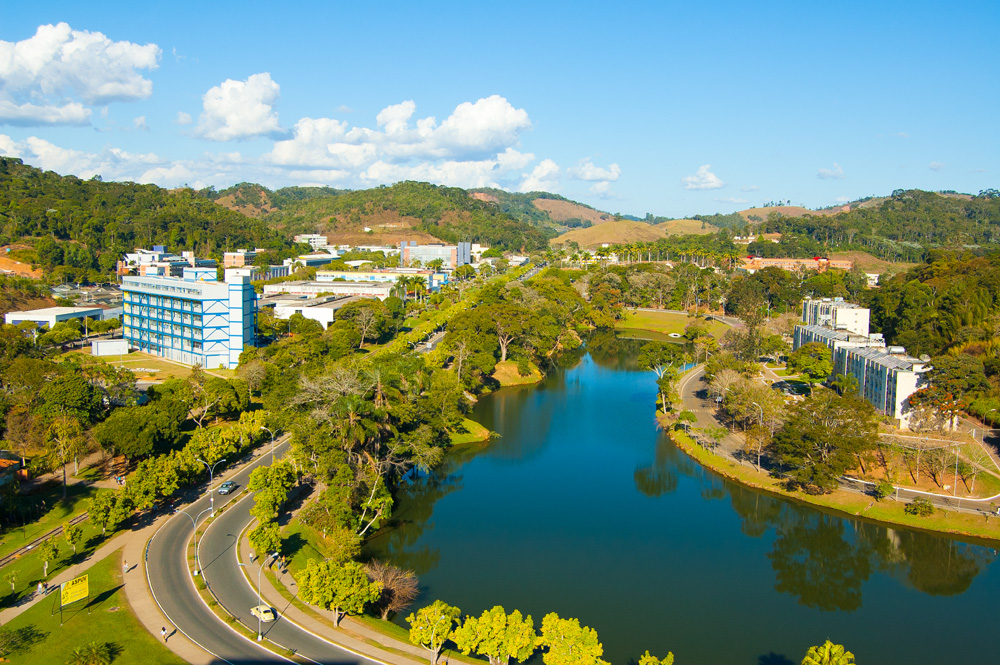
\includegraphics[scale=0.7]{./capitulos/cap01/ufv.jpg}
\end{figure}
\section{Seção nova}
\lipsum[2-3]
%%%% APAGAR O EXEMPLO ACI

%%%% REFERÊNCIAS
\bibliography{referencias.bib}
\bibliographystyle{apalike}
\end{document}

\documentclass[12pt]{report}
\usepackage[utf8]{inputenc}
\usepackage[brazilian,brazil]{babel}
\usepackage{fancyhdr,setspace,float,graphicx,lscape,array,longtable,colortbl,amsmath,amssymb,booktabs,multirow,hyperref,pdfpages,tocloft,titlesec,lipsum,natbib}
\usepackage[sectionbib]{chapterbib}

\begin{document}
\chapter{Título do capítulo}
\lipsum[2-4] \lipsum[1]
\begin{table}[]
\centering
\caption{Minha tabela}
\label{my-label}
\begin{tabular}{lll}
1 & a & s \\ \hline
1 & a & x \\
2 & z & s
\end{tabular}
\end{table}
\section{Seção nova}
\lipsum[2-3]
De acordo com \cite{Rodrigues2016} e \cite{kopka2004guide}.



%%%% REFERÊNCIAS
\bibliography{referencias.bib}
\bibliographystyle{apalike}
\end{document}



\documentclass[12pt]{report}
\usepackage[utf8]{inputenc}
\usepackage[brazilian,brazil]{babel}
\usepackage{fancyhdr,setspace,float,graphicx,lscape,array,longtable,colortbl,amsmath,amssymb,booktabs,multirow,hyperref,pdfpages,tocloft,titlesec,lipsum,natbib}
\usepackage[sectionbib]{chapterbib}


\begin{document}
\chapter{Outro título}
\lipsum[2-10] \citep{Rodrigues2016}

%%%% REFERÊNCIAS
\bibliography{referencias.bib}
\bibliographystyle{apalike}
\end{document}


% se necessário acrescente outros capítulos, por exemplo:
% \input{capitulos/cap04/cap04}

%****************************************************************************************************
% Análises estatísticas em pdf
% Descomente e coloque o nome do seu arquivo
%\includepdf[pages=-]{nome_do_arquivo.pdf}
%****************************************************************************************************
  
\end{document}
